%!TEX TS-program = xelatex
%!TEX encoding = UTF-8 Unicode
%
% 本文為 LaTeX 快速入門, 中文使用 xeCJK (XeLaTeX) 配上 cwTeX Q Fonts 的五套字型。
% 另外, 請注意 minted 這個套件需要特別安裝, 請參考相關文件說明。
%

\documentclass[12pt]{report}
\usepackage[a4paper]{geometry} 
\usepackage{graphicx}
\usepackage{amssymb, amsmath, amsthm}		% AMS 標準套件
\usepackage{booktabs}						% 表格線條
\usepackage{hyperref}							% 使用 \url 等指令
\usepackage{titlesec} 							% 美化章節標題套件
\usepackage{minted}							% 程式碼 (注意這要特別安裝)
\usepackage{tikz}								% 使用 tikz 套件

\graphicspath{{images/}} 						% 設定圖形路徑


% === 中文 xeCJK 設定 ===
\usepackage{xeCJK}
\setCJKmainfont[BoldFont={cwTeX Q Hei Bold}]{cwTeX Q Ming Medium} % 設預設中文字型及預設粗體
\setCJKfamilyfont{kai}{cwTeX Q Kai Medium}			    	% 楷書	      			
\setCJKfamilyfont{hei}{cwTeX Q Hei Bold}				% 黑體
\setCJKfamilyfont{ming}{cwTeX Q Ming Medium}			% 明體
\setCJKfamilyfont{yuan}{cwTeX Q Yuan Medium}			% 圓體
\setCJKfamilyfont{fsong}{cwTeX Q Fangsong Medium}		% 仿宋體

\newcommand{\kai}[1]{{\CJKfamily{kai}#1}}   			% 用 \kai{使用楷書}
\newcommand{\hei}[1]{{\CJKfamily{hei}#1}}   			% 用 \hei{使用黑體}
\newcommand{\ming}[1]{{\CJKfamily{ming}#1}}		% 用 \ming{使用明體}
\newcommand{\yuan}[1]{{\CJKfamily{yuan}#1}}		% 用 \yuan{使用圓體}
\newcommand{\fsong}[1]{{\CJKfamily{fsong}#1}}		% 用 \fsong{使用仿宋體}

\setromanfont[Mapping=tex-text]{Times} 					% 指定英文字型, 並用 LaTeX 引號
\setsansfont[Scale=MatchLowercase,Mapping=tex-text]{Arial}	% 指定無描邊字型
\setmonofont[Scale=MatchLowercase]{Courier} 				% 指定等寛字型



% === 排版設定 ===
\setlength{\parindent}{0pt}  	% 設定縮排
\linespread{1.2} 				% 設定行距
\setlength{\parskip}{15pt} 		% 設定段落間距


% === 自訂指令 ===
\newcommand{\cmd}{\texttt}
\renewcommand\contentsname{目~錄~}
\renewcommand\listfigurename{圖~目~錄}
\renewcommand\listtablename{表~目~錄}


% === 章節標題 (配合 titlesec) ===
\titleformat{\chapter}[display]
	{\bf\Large}
	{\filleft 第 \thechapter\ 章}
	{1ex}
	{\Huge\titlerule
	 \vspace{2ex}%
	 \filright}
	[\vspace{2ex}%
	 \titlerule]

%%%%%%%%
%
% 本文特有的規定
%
%%%%%%%%
%
\newtheorem{thm}{Theorem}
\newtheorem{thm1}{Theorem}[section]
\newtheorem{thm2}{Theorem}
\newtheorem{lem}{Lemma}
\newtheorem{thm3}{Theorem}
\newtheorem{lem3}[thm3]{Lemma}
\newtheorem*{mainthm}{Main Theorem}
\theoremstyle{plain}
\newtheorem{thms}{Theorem}
\theoremstyle{definition}
\newtheorem{defns}{Definition}
\theoremstyle{remark}
\newtheorem{rmks}{Remark}
\newminted{latex}{frame=single}

\title{\hei{\LaTeX{} 的快速入門}}
\author{蔡炎龍\\ 政治大學應用數學系}
\date{2014 年版}

\begin{document}
\maketitle

\tableofcontents
%%%
\chapter{前言}
%
\section{這份文件的目的}
這份文件是希望提供有心想學 \LaTeX{} 的人, 一份快速入門的文件。我心目中的主要讀者是研究生, 所以我們會以最快的速度去討論怎麼樣把一篇論文完成, 包括 Bib\TeX{} 的論文管理。但另一方面來說, 我又希望可以更廣泛的讓 \LaTeX{} 帶入一般文件處理, 而不只是在論文上面, 所以我會將中文 \LaTeX{} 一併帶入。好在現在要用 \LaTeX{} 編輯中文文件已比以前簡單太多, 我們其實不用特別多安裝什麼, 就可以使用!

中文方面我們採用 Xe\LaTeX, 這套系統的好處是可以用自己電腦裡的字型! 壞處是要特別用 Xe\LaTeX{} 編譯, 而且如果有共同合作者就要小心系統中是否有相同的字型。我們建議使用 cwTeX Q 五套字型, 不過當然個人使用你大可自由使用你想要的字型。

本文件不介紹安裝的問題, 安裝請參考我另一份文件《中英文 \LaTeX{} 安裝與應用》, 本篇假設大家是安裝完成了。如果是在政大, 可以到應用數學系電腦室, 我們已經設好我們這篇文章討論應有的 \LaTeX{} 環境。

另外, 為了順利的使用 \LaTeX, 你應該要有個順手的純文字編輯器。我個人推薦的編輯器如下:
\begin{itemize}
\item TeXWorks (所有平台都有)
\item Vim (Unix-like 系統, 如果自認 Geek 級使用者)
\item TeXShop (Mac OS X, 事實上我最偏好這一個)
\end{itemize}

我們只準備使用 PDF\LaTeX{} 和 Xe\LaTeX{}, 這樣我們所有的 \LaTeX{} 檔, 都直接產生 PDF 文件。中文編碼我們只準備使用 UTF-8, 這除了是個潮流, 也讓英文和中文基本上用的流程是完全一樣。
%
\section{版本資訊}
這份文件是在 2007 年 7 月 16 日完成第一版初稿, 7 月 18 日改用 Xe\LaTeX{} 進行改版。2013 年再做修正, 2014 年在 GitHub 上公開所有檔案。

%%%
\chapter{\LaTeX{} 極速入門}
很多人說 \LaTeX{} 很難, 其實 \LaTeX{} 實在沒什麼難的。我們只不過是做一個純文字檔, 存成 \cmd{.tex} 這樣的檔案, 然後使用 \cmd{pdflatex} 這個指令, 馬上就產生一篇高品質的 PDF 文件。
%
\begin{center}
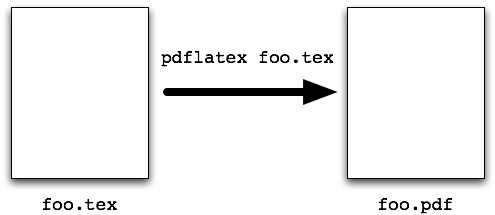
\includegraphics[width=10cm]{pdflatex.png}
\end{center}

我們這裡很快的來看一下這個 \cmd{.tex} 的純文字檔應該長什麼樣子。
%
\section{最簡單的 \LaTeX{} 文件}
最簡單的 \LaTeX{} 檔案是長這個樣子。
%
\begin{latexcode}
\documentclass{article}
\begin{document}

% 內文, 文章的內容

\end{document}
\end{latexcode}
可以試打一些內容進去看看, 存成 \cmd{.tex} 檔, 再用 \cmd{pdflatex} 編譯。要注意目前還不能用中文。
%
\section{完整的 \LaTeX{} 格式}
一份完整的 \LaTeX{} 文件的架構大概如下。
\begin{latexcode}
\documentclass{article}

% 設定區, 我們還不會

\title{文章的標題}
\author{作者}

\begin{document}
\maketitle

% 內文, 文章的內容

\end{document}
\end{latexcode}
框起來的部份就是我們需要打字進去的地方。你可以試打一些東西進去, 然後 \LaTeX{} 會自動幫你印出標題、作者、有分節的文件。是不是非常容易? \LaTeX{} 的一個特性就是, 你可以{\bf 專注在文章的內容上, 要美化什麼的可以最後慢慢調}。
%
%
\chapter{\LaTeX{} 數學式子基礎}

\section{數學模式}
很多人聽說 \LaTeX, 都是聽說它對數學符號處理功力很強。我們來看看要怎麼打入數學符號。\LaTeX{} 有兩種數學模式, 分別是:
\begin{itemize}
\item 隨文模式 (\cmd{inline mode})
\item 展示模式 (\cmd{display mode})
\end{itemize}
我們來看看怎麼樣使用。
\subsubsection{隨文模式}
所謂隨文模式就是數學式子要插在文中, 使用的方式是把數學式子放入兩個 \$ 的符號中。比方說下面這個例子:

\begin{center}
\begin{minipage}[t]{0.38\linewidth}\vfill
The formula $f(x)=x^3 - 2x +6$ is important in this case.
\end{minipage}
\begin{minipage}[t]{0.58\linewidth}
\begin{latexcode}
The formula $f(x)=x^3 - 2x +6$ is 
important in this case.
\end{latexcode}
\end{minipage}
\end{center}

\section{展示模式}
所謂展示模式的數學式子, 是把數學式{\bf 獨立、置中}表示。展示模式有很多下指令的方式, 我們可以把數學式子用 ``\cmd{\$\$ \ldots \$\$}'', ``\cmd{$\backslash$[ \ldots $\backslash$]}'', 或 ``\cmd{$\backslash$begin\{equation\} \ldots $\backslash$end\{equation\}}'' 等方式表示, 比方說

\begin{center}
\begin{minipage}[t]{0.38\linewidth}\vfill
The formula
\[
f(x)=x^3 - 2x +6
\]
is important in this case.
\end{minipage}
\begin{minipage}[t]{0.58\linewidth}
\begin{latexcode}
The formula
\[
f(x)=x^3 - 2x +6
\]
is important in this case.
\end{latexcode}
\end{minipage}
\end{center}

\section{好用的 \LaTeX{} 工具}

%
\subsection{MyScript 的 Web Equation}

MyScript 是一個「手寫辨識」的程式庫, 他們做了網路示範版本。你可以到他們示範網頁:

\url{http://webdemo.visionobjects.com/portal.html?locale=en}

\begin{center}
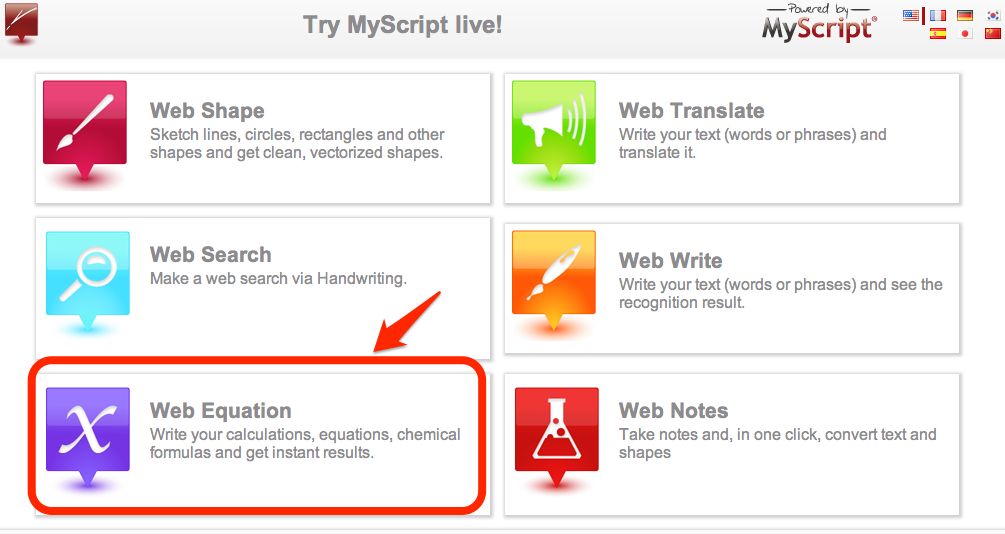
\includegraphics[scale=0.4]{webequation01}
\end{center}

我們要用的是 Web Equation。然後你就用手寫出一個數學式子, Web Equation 辨識輸出 \LaTeX{} 碼, 而且即時預覽, 讓你知道辨識結果有沒有問題!

\begin{center}
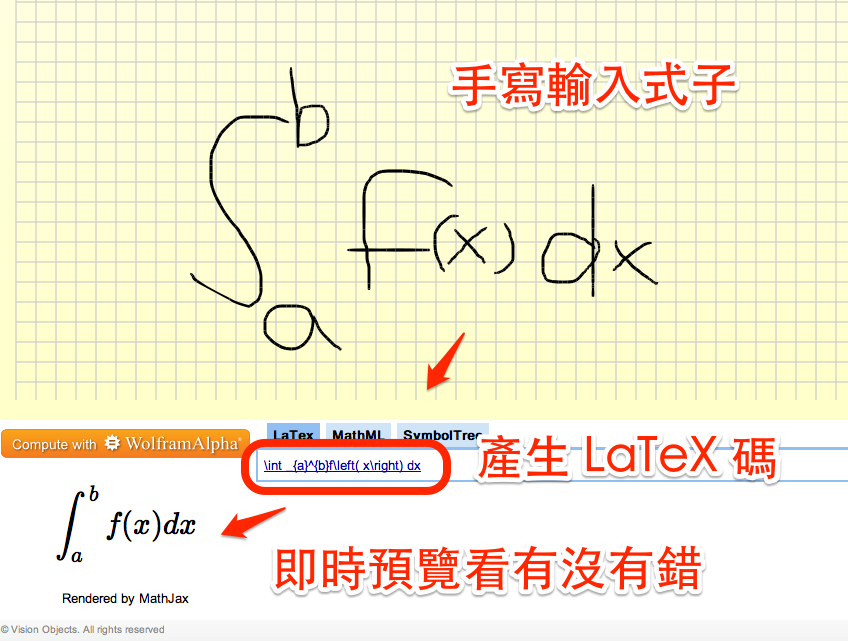
\includegraphics[scale=0.4]{webequation02}
\end{center}


%
\subsection{Detexify 手寫符號}

接著我們介紹和 Web Equation 有點像, 但這次著重在符號上。我們常常會碰到某個 \LaTeX{} 符號不知怎麼打, 最容易的方式當然是寫出我們要的符號, 電腦就告訴我們怎麼下指令! Detexify 就是做這樣的工作:

\url{http://detexify.kirelabs.org}

你手寫一個符號, Detexify 會列出它覺得長得像的, 還告訴你需不需要特別套件、要在文字模式還是數學模式下使用。

\begin{center}
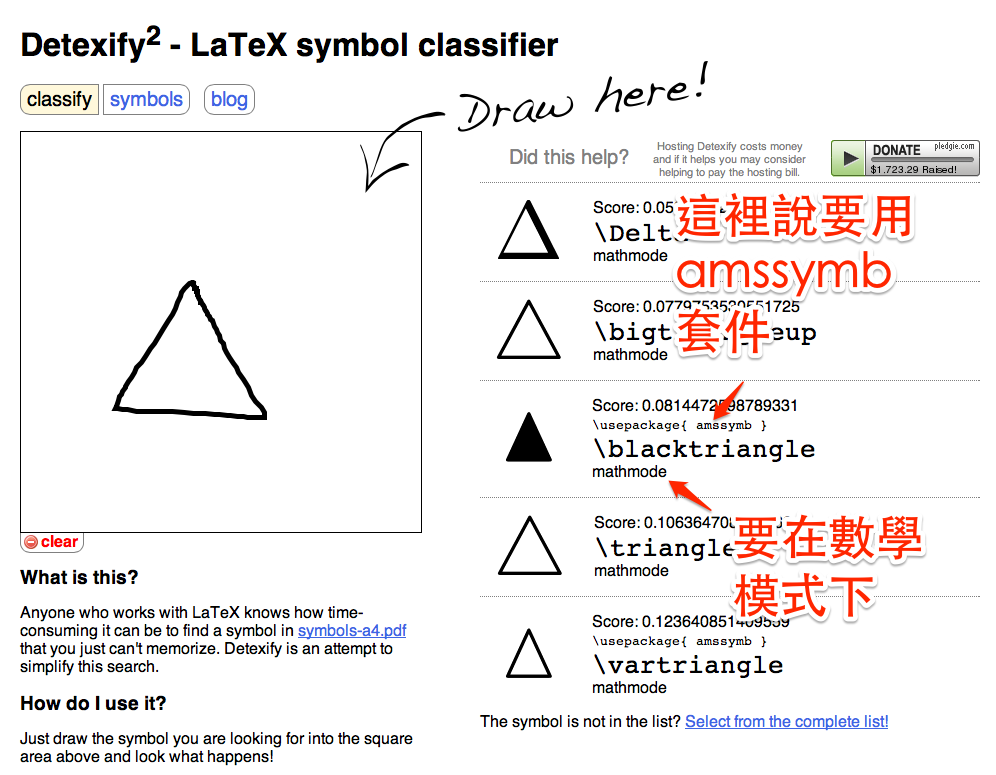
\includegraphics[scale=0.4]{detexify}
\end{center}


%
\subsection{\LaTeX{} 符號大全集}

如果你有什麼符號, 實在不知怎麼打出來, 用了我們介紹的方式也找不到。現在介紹一個殺手鐧 -- Scott Pakin 的 ``The Comprehensive \LaTeX{} Symbol List''。你可以在這裡下載:

\url{http://www.ctan.org/tex-archive/info/symbols/comprehensive/}

這有完整到什麼程度呢? 完整到你沒有想過 \LaTeX{} 可以打出的「符號」都可以找到!

%
\chapter{使用 Xe\LaTeX{} 來打中文}
%
\section{Xe\LaTeX{} 的快速入門}
前一章介紹的 CJK-\LaTeX{} 麻煩的地方是要安裝特別的字型, 我們可不可以直接使用系統上的字型呢? 答案是可以的! 只要使用 Xe\LaTeX, 你可以使用自己電腦裡的字型。

Xe\LaTeX{} 是由 Jonathan Kew 開發的, 中國南開大學孫文昌教授為 Xe\LaTeX{} 寫了對中文使用者很方便的 xeCJK 套件, 省了很多設定上的麻煩。所以我們主要介紹 xeCJK 的用法。在編譯時還是要用 Xe\LaTeX{} 編譯。

我們首先要選擇系統裡的一個字型, 找到它的名稱, 接著就照以下範例打, 就可以完全不用裝字型 (或依《中英文 \LaTeX{} 安裝與應用》安裝 cwTeX-Q 字型), 馬上使用中文 \LaTeX! 現在假設我們想用 cw\TeX-Q 的明體字 (\cmd{cwTeX Q Ming Medium}), 我們可以這樣做:

\begin{latexcode}
\documentclass{article}

\usepackage{xeCJK}
\setCJKmainfont{cwTeX Q Ming Medium}

\begin{document}

文章內容如一般 \LaTeX, 還可打中文!

\end{document}
\end{latexcode}

出來的結果如下:

\framebox[10cm]{
文章內容如一般 \LaTeX, 還可打中文!
}

%

所以基本上就是一般的 \LaTeX, 只有先引用套件

\begin{latexcode}
\usepackage{xeCJK}
\end{latexcode}

然後再設定我們要用的字型

\begin{latexcode}
\setCJKmainfont{cwTeX Q Ming Medium}
\end{latexcode}

就可以了!

唯一要小心是在編譯時, 我們要選用 Xe\LaTeX{} 編譯。比方說, 我們的 \LaTeX{} 檔叫 \cmd{foo.tex}, 那我們就可以這樣編譯:

\begin{latexcode}
xelatex foo.tex
\end{latexcode}

%
\section{Xe\LaTeX{} 中文字型設定}

我們打文章, 很可能正常的字體用明體, 粗體字用黑體, 這樣 Xe\LaTeX{} 下要怎麼做呢? 答案是我們在設定中文字型時可以加一些參數。比方說

\begin{latexcode}
\setCJKmainfont[BoldFont={cwTeX Q Hei Bold}]
{cwTeX Q Ming Medium}
\end{latexcode}

這樣主要的字體仍然是使用 \cmd{cwTeX Q Ming Medium} (明體), 而粗體字會用 \cmd{cwTeX Q Hei Bold}。

我們看以下的例子。

\begin{center}
\begin{minipage}[t]{0.38\linewidth}\vfill
這裡就是最{\bf{重要}}的地方。
\end{minipage}
\begin{minipage}[t]{0.58\linewidth}

\begin{latexcode}
這裡就是最{\bf{重要}}的地方。
\end{latexcode}
\end{minipage}
\end{center}

我們更可以再設用楷書為「斜體」字, 如

\begin{latexcode}
\setCJKmainfont[BoldFont={cwTeX Q Hei Bold}, 
ItalicFont={cwTeX Q Kai Medium}]{cwTeX Q Ming Medium}
\end{latexcode}

%
\section{Xe\LaTeX{} 英文字型設定}
Xe\LaTeX{} 當然不只可以用系統的中文字型, 英文字型也可以任意選用! 現在假設我們中文字型設好了, 可不可以顯示英文時用英文字型呢? 當然可以! 我們只要設

\begin{latexcode}
\setromanfont{Times} 
\end{latexcode}

就可以把英文字型設成 ``Times'' 字型。但這樣設我們用一般英文 \LaTeX{} 打標點等方式會看來怪怪的。這時我們可以設

\begin{latexcode}
\setromanfont[Mapping=tex-text]{Times} 
\end{latexcode}

就好了。我們還可以分別設無描邊字型、等寬字型等等, 現舉例如下:

\begin{latexcode}
\setromanfont[Mapping=tex-text]{Times}
\setsansfont[Scale=MatchLowercase, Mapping=tex-text]{Arial}
\setmonofont[Scale=MatchLowercase]{Courier} 
\end{latexcode}

新用的 \cmd{Scale} 參數設 ``MatchLowercase'' 是保證各字型小寫的 ``x'' 是一樣大小的。

% \kai 等等?

%%%
\chapter{使用 AMS-\LaTeX}

\section{引入 AMS-\LaTeX}
AMS 美國數學學會的 \LaTeX{} 套件已然成為一種標準。通常會用到的有三個套件:
\begin{itemize}
\item \cmd{amssymb}: 提供一些原本 \LaTeX{} 沒有的符號, 比方說 $\mathbb{R}$, $\mathbb{C}$, 等等。
\item \cmd{amsmath}: 提供一些好用的環境, 比方說 \cmd{align} 環境等等。
\item \cmd{amsthm}: 提供比較好的使用定理、定義等的環境。
\end{itemize}
如果使用一般的 \cmd{article class}, 建議每次都把三個套件讀進來:

\begin{latexcode}
\usepackage{amssymb, amsmath, amsthm}
\end{latexcode}

%
\section{使用 AMS Article Class}
使一個使用 AMS-\LaTeX{} 的方式是使用 AMS 提供的個文章類型, 叫 AMS Article。要使用就是設定使用 \cmd{amsart}:

\begin{latexcode}
\documentclass{amsart}
\end{latexcode}

它會自動讀入 \cmd{amsmath}, \cmd{amsthm} 兩個套件, 和部份 \cmd{amssymb} 套件 (比方說有 $\mathbb{R}$)。如果需要全套的 \cmd{amssymb},  還是要自行讀入:

\begin{latexcode}
\usepackage{amssymb}
\end{latexcode}

%%%
\chapter{定理環境的使用}\label{S:thm}
我們寫數學文章, 總會出現定義, 定理, 證明等等。我們在 \LaTeX{} 要處理這些東西是很容易的。

%
\section{基本定理環境}
在設定區設定:
\begin{minted}[frame=single, framerule=1pt]{latex}
\newtheorem{thm}{Theorem}
\end{minted}
意思是我們要先建一個新的定理環境, 叫做 \cmd{thm}, 顯示時標示為 ``Theorem''。比方說:

\begin{center}
\begin{minipage}[t]{0.38\linewidth}\vfill
\begin{thm}
The statements of the theorem.
\end{thm}
\end{minipage}
\begin{minipage}[t]{0.58\linewidth}

\begin{latexcode}
\begin{thm}
The statements of the theorem.
\end{thm}
\end{latexcode}
\end{minipage}
\end{center}

\section{定理的編號}
你可以發現定理的編號會自動從 1, 2, 3, 等等編下去。但是有時我們要依節次來標, 比方說第一節的第一個定理的編號是 1.1, 然後 1.2, 1.3, 這樣下去, 要怎麼做呢? 很容易, 加個 \cmd{section} 參數就好。比如說在設定時我們設:

\begin{latexcode}
\newtheorem{thm}{Theorem}[section]
\end{latexcode}

那麼在本節 (第 \ref{S:thm} 節) 使用定理環境會變成下面這個樣子。

\begin{center}
\begin{minipage}[t]{0.38\linewidth}\vfill
\begin{thm1}
The statements of the theorem.
\end{thm1}
\end{minipage}
\begin{minipage}[t]{0.58\linewidth}

\begin{latexcode}
\begin{thm}
The statements of the theorem.
\end{thm}
\end{latexcode}
\end{minipage}
\end{center}

我們如果定了兩個定理環境, 他們原本是互不相干的, 所以會各自編號。比如說如果我們有設了 \cmd{thm}, \cmd{lem} 兩個定理環境:

\begin{latexcode}
\newtheorem{thm}{Theorem}
\newtheorem{lem}{Lemma}
\end{latexcode}

引用起來會是像這樣子:

\begin{center}
\begin{minipage}[t]{0.38\linewidth}\vfill
\begin{lem}
The statements of the lemma.
\end{lem}
\begin{thm2}
The statements of the theorem.
\end{thm2}
\end{minipage}
\begin{minipage}[t]{0.58\linewidth}
\begin{latexcode}
\begin{lem}
The statements of the lemma.
\end{lem}
\begin{thm}
The statements of the theorem.
\end{thm}
\end{latexcode}
\end{minipage}
\end{center}

這樣子的編號方式, 我們無法知道 Lemma 7 和 Theorem 3 倒底是哪一個先出現, 哪一個後出現。要用統一的編號。比方說引理 1 之後是定理 2 等等, 就要用下面的方式宣告定理環境。

\begin{latexcode}
\newtheorem{thm}{Theorem}
\newtheorem{lem}[thm]{Lemma}
\end{latexcode}

請比較和以前有什麼不一樣。

\begin{center}
\begin{minipage}[t]{0.38\linewidth}\vfill
\begin{lem3}
The statements of the lemma.
\end{lem3}
\begin{thm3}
The statements of the theorem.
\end{thm3}
\end{minipage}
\begin{minipage}[t]{0.58\linewidth}
\begin{latexcode}
\begin{lem}
The statements of the lemma.
\end{lem}
\begin{thm}
The statements of the theorem.
\end{thm}
\end{latexcode}
\end{minipage}
\end{center}

最後, 如果需要完全沒有編號的定理環境, 就要像下面這樣加上星號。
\begin{latexcode}
\newtheorem*{mainthm}{Main Theorem}
\end{latexcode}

\begin{center}
\begin{minipage}[t]{0.38\linewidth}\vfill
\begin{mainthm}
The statements of the theorem.
\end{mainthm}
\end{minipage}
\begin{minipage}[t]{0.58\linewidth}
\begin{latexcode}
\begin{mainthm}
The statements of the theorem.
\end{mainthm}
\end{latexcode}
\end{minipage}
\end{center}

%
\section{不同定理風格 (amsthm)}
使用 \cmd{amsthm}, 可以指定三種不同的定理風格: \cmd{plain}, \cmd{definition}, 和 \cmd{remark}。使用方式是在定義定理環境之前, 先下達:
\begin{latexcode}
\theoremstyle{[定理風格]}
\end{latexcode}

舉例來說, 假設我們定義下列的定理環境:
\begin{latexcode}
\theoremstyle{plain}
\newtheorem{thm}{Theorem}

\theoremstyle{definition}
\newtheorem{defn}{Definition}

\theoremstyle{remark}
\newtheorem{rmk}{Remark}
\end{latexcode}

會產生如下的效果。

\begin{center}
\begin{minipage}[t]{0.38\linewidth}\vfill
\begin{thms}
The statements of the theorem.
\end{thms}
\begin{defns}
The statements of the definition.
\end{defns}
\begin{rmks}
The statements of the remark.
\end{rmks}
\end{minipage}
\begin{minipage}[t]{0.58\linewidth}
\begin{latexcode}
\begin{thm}
The statements of the theorem.
\end{thm}
\begin{defn}
The statements of the definition.
\end{defn}
\begin{rmk}
The statements of the remark.
\end{rmk}
\end{latexcode}
\end{minipage}
\end{center}

%
\section{定理的引用}
我們會引用到的定理, 就用 \cmd{$\backslash$label$\{$\fbox{\rm 引用代碼}$\}$} 來標記。比方說

\begin{center}
\begin{minipage}[t]{0.38\linewidth}\vfill
\begin{thm}\label{T:major}
The statements of the theorem.
\end{thm}
\end{minipage}
\begin{minipage}[t]{0.58\linewidth}
\begin{latexcode}
\begin{thm}\label{T:major}
The statements of the theorem.
\end{thm}
\end{latexcode}
\end{minipage}
\end{center}

要引用的時候, 就是用  $\sim\backslash$\cmd{ref$\{$\fbox{\rm 引用代碼}$\}$}:

\begin{center}
\begin{minipage}[t]{0.38\linewidth}\vfill
Please refer to Theorem~\ref{T:major}.
\end{minipage}
\begin{minipage}[t]{0.58\linewidth}
\begin{latexcode}
Please refer to 
Theorem~\ref{T:major}.
\end{latexcode}
\end{minipage}
\end{center}

%%%
\chapter{插入圖片}
%
\section{插入圖片的基本方法}
這裡建議使用 \cmd{graphicx} 套件:
\begin{latexcode}
\usepackage{graphicx}
\end{latexcode}

假設我們要插入 \cmd{pic.png} 這個圖檔, 使用
\begin{latexcode}
\includegraphics[width=5cm]{pic.png}
\end{latexcode}

即可。自然, \cmd{width} 是可依你需要設定的。建議使用的圖檔格式為:
\begin{Verbatim}[frame=single, framerule=1pt]
.png, .pdf, .jpg
\end{Verbatim}
%
\section{圖片置中}
要把圖片置中, 使用 \cmd{center} 環境即可:
\begin{latexcode}
\begin{center}
\includegraphics[width=5cm]{pic.png}
\end{center}
\end{latexcode}
%
\section{figure 的使用方法}
上面的圖形基本上是在那插入, 就會放在那裡。但正式排版中, 常會依版面情況調整位置, 且會有提示文字。這時要使用 \cmd{figure} 環境。一般要置中, 又有說明的圖會這樣引用:
\begin{latexcode}
\begin{figure}
\begin{center}
\includegraphics[width=圖形寬度]{檔案名稱}
\end{center}
\caption{圖形的文字說明}
\end{figure}
\end{latexcode}

\LaTeX{} 會幫你把圖形放在它認為合適的地方。如果你對放的位置很有意見, 可以加入 \cmd{h}, \cmd{t}, \cmd{b}, 或 \cmd{p} 等參數改變。比方說使用
\begin{latexcode}
\begin{figure}[h] ... 
\end{latexcode}

這些參數代表你希望放置的位置分別是:

\begin{itemize}
\item \cmd{h}: 放在此處
\item \cmd{t}: 放在頂端
\item \cmd{b}: 放在底端
\item \cmd{p}: 在本頁
\end{itemize}

事實上你也可以同時用 \cmd{[htbp]}, 這是告訴 \LaTeX{} 你希望放在這一頁, 但到底怎麼放讓 \LaTeX{} 自己「看著辦」。
%
\section{圖形的引用}
圖形的引用其實和定理引用一樣。你只要在想引用的圖提示文字加上 $\backslash$\cmd{label}, 比方說:
\begin{latexcode}
\caption{圖形的提示文字}\label{引用代碼}
\end{latexcode}

要引用時則如下範例:
\begin{latexcode}
參考圖~\ref{引用代碼}...
\end{latexcode}

就可以了。

%%%
\chapter{列表}

我們這裡介紹怎麼樣在 \LaTeX{} 使用文書處理常用的列表。

\section{基本列表}
要分點列表的基本方式如下:

\begin{center}
\begin{minipage}[t]{0.38\linewidth}\vfill
\begin{itemize}
\item 微積分
\item 高等微積分
\item 線性代數
\end{itemize}
\end{minipage}
\begin{minipage}[t]{0.58\linewidth}
\begin{latexcode}
\begin{itemize}
\item 微積分
\item 高等微積分
\item 線性代數
\end{itemize}
\end{latexcode}
\end{minipage}
\end{center}

\section{數字列表}
我們再看要以 1, 2, 3 等標示的列表怎麼做。

\begin{center}
\begin{minipage}[t]{0.38\linewidth}\vfill
\begin{enumerate}
\item 微積分
\item 高等微積分
\item 線性代數
\end{enumerate}
\end{minipage}
\begin{minipage}[t]{0.58\linewidth}
\begin{latexcode}
\begin{enumerate}
\item 微積分
\item 高等微積分
\item 線性代數
\end{enumerate}
\end{latexcode}
\end{minipage}
\end{center}

\section{定義型列表}
第三種定義型列表使用方式如下。

\begin{center}
\begin{minipage}[t]{0.38\linewidth}\vfill
\begin{description}
\item [微積分] 大一必修
\item [高等微積分] 大二必修
\item [線性代數] 大二必修
\end{description}
\end{minipage}
\begin{minipage}[t]{0.58\linewidth}
\begin{latexcode}
\begin{description}
\item [微積分] 大一必修
\item [高等微積分] 大二必修
\item [線性代數] 大二必修
\end{description}
\end{latexcode}
\end{minipage}
\end{center}

%%%
\chapter{陣列和表格}
%
\section{陣列的使用}
陣列就是如同矩陣型的排列。我們可以看一下一個例子。

\begin{center}
\begin{minipage}[t]{0.38\linewidth}\vfill
\[
\begin{array}{ccc}
1 & 2 & 3 \\
4 & 5 & 6 \\
7 & 8 & 9
\end{array}
\]
\end{minipage}
\begin{minipage}[t]{0.58\linewidth}
\begin{latexcode}
\[
\begin{array}{ccc}
1 & 2 & 3 \\
4 & 5 & 6 \\
7 & 8 & 9
\end{array}
\]
\end{latexcode}
\end{minipage}
\end{center}

這裡要說明一下。

\begin{latexcode}
\begin{array}{ccc}
\end{latexcode}

是表示要用陣列, 這個陣列有三行, 每一行都要對齊中間 (\cmd{c})。對齊的方式有三種選擇:
\begin{itemize}
\item \cmd{c}: 對齊中間
\item \cmd{l}: 對齊左邊
\item \cmd{r}: 對齊右邊
\end{itemize}

我們要一列一列輸入, 要換行時用 ``$\backslash\backslash$'' 換行, 每一欄用 ``\&'' 隔開。
%
\section{表格的使用方式}
表格的使用方式非常接近陣列的使用。

\begin{center}
\begin{minipage}[t]{0.38\linewidth}\vfill
\begin{tabular}{ccc}
item 1 & item 2 & item 3 \\
1 & 2 & 3 \\
4 & 5 & 6
\end{tabular}
\end{minipage}
\begin{minipage}[t]{0.58\linewidth}
\begin{latexcode}
\begin{tabular}{ccc}
item 1 & item 2 & item 3 \\
1 & 2 & 3 \\
4 & 5 & 6
\end{tabular}
\end{latexcode}
\end{minipage}
\end{center}

如果要加橫線, 加入 $\backslash$\cmd{hline}:

\begin{center}
\begin{minipage}[t]{0.38\linewidth}\vfill
\begin{tabular}{ccc} \hline
item 1 & item 2 & item 3 \\ \hline
1 & 2 & 3 \\ \hline
4 & 5 & 6 \\ \hline
\end{tabular}
\end{minipage}
\begin{minipage}[t]{0.58\linewidth}
\begin{latexcode}
\begin{tabular}{ccc} \hline
item 1 & item 2 & item 3 \\ \hline
1 & 2 & 3 \\ \hline
4 & 5 & 6 \\ \hline
\end{tabular}
\end{latexcode}
\end{minipage}
\end{center}

加直線更方便, 在對齊設定那加就可以了:

\begin{center}
\begin{minipage}[t]{0.38\linewidth}\vfill
\begin{tabular}{|c|c|c|} \hline
item 1 & item 2 & item 3 \\ \hline
1 & 2 & 3 \\ \hline
4 & 5 & 6 \\ \hline
\end{tabular}
\end{minipage}
\begin{minipage}[t]{0.6\linewidth}
\begin{latexcode}
\begin{tabular}{|c|c|c|} \hline
item 1 & item 2 & item 3 \\ \hline
1 & 2 & 3 \\ \hline
4 & 5 & 6 \\ \hline
\end{tabular}
\end{latexcode}
\end{minipage}
\end{center}

%
\section{一般的括號和會變大的括號}
在 \LaTeX{} 裡, 要打出小括號到大括號方法如下:
\begin{itemize}
\item 小括號: \cmd{(\  )}
\item 中括號: \cmd{[\  ]}
\item 大括號: $\backslash\{\  \backslash\}$
\end{itemize}

問題是如果你想打一個矩陣, 配合 \cmd{array} 使用, 會出現一個好笑的結果:

\begin{center}
\begin{minipage}[t]{0.38\linewidth}\vfill
\[
(\begin{array}{ccc}
1 & 2 & 3 \\
4 & 5 & 6 \\
7 & 8 & 9
\end{array})
\]
\end{minipage}
\begin{minipage}[t]{0.58\linewidth}
\begin{latexcode}
\[
(\begin{array}{ccc}
1 & 2 & 3 \\
4 & 5 & 6 \\
7 & 8 & 9
\end{array})
\]
\end{latexcode}
\end{minipage}
\end{center}

要改正這個缺點, 我們要用「可自調大小的括號」。方式很簡單, 在左邊的括號前加 $\backslash$\cmd{left}, 右邊加 $\backslash$\cmd{right} 就可以。比方說:

\begin{center}
\begin{minipage}[t]{0.38\linewidth}\vfill
\[
\left(\begin{array}{ccc}
1 & 2 & 3 \\
4 & 5 & 6 \\
7 & 8 & 9
\end{array}\right)
\]
\end{minipage}
\begin{minipage}[t]{0.58\linewidth}
\begin{latexcode}
\[
\left(\begin{array}{ccc}
1 & 2 & 3 \\
4 & 5 & 6 \\
7 & 8 & 9
\end{array}\right)
\]
\end{latexcode}
\end{minipage}
\end{center}

%
\section{陣列和括號的應用}

注意前面「會變大小的括號」是一定要成對出現的。如果我們已經用了 $\backslash$\cmd{left}, 一定要有 $\backslash$\cmd{right}。不過, 我們其實可以只要一邊, 比方說左邊的括號, 而右邊可用 $\backslash$\cmd{right}. 表示不要顯示任何括號。
我們來看一個應用:

\begin{center}
\begin{minipage}[t]{0.38\linewidth}\vfill
\[
|x| = \left\{
\begin{array}{rr}
 x, & \mbox{if $x \geq 0$} \\
-x, & \mbox{if $x < 0$}
\end{array} \right.
\]
\end{minipage}
\begin{minipage}[t]{0.58\linewidth}
\begin{latexcode}
\[
|x| = \left\{
\begin{array}{rr}
 x, & \mbox{if $x \geq 0$} \\
-x, & \mbox{if $x < 0$}
\end{array} \right.
\]
\end{latexcode}
\end{minipage}
\end{center}

這裡我們新學一件事, 那就是{\bf 如果數學式中我們要打入一些純文字, 可以用 $\backslash$\cmd{mbox} 指令}。而在 $\backslash$\cmd{mbox} 裡面的是純文字, 所以再打數學符號就要加上錢的符號了。

%%%
\chapter{Bib\TeX{} 入門}
%
\section{為什麼要用 Bib\TeX?}
使用 Bib\TeX{} 並不是在 \LaTeX{} 下引用論文唯一方式。開始的時候, 用 Bib\TeX{} 可能還會覺得比較麻煩, 因為你為了論文, 還要建立一個 \cmd{.bib} 純文字檔, 內容是你要引用的論文資訊。我們為什麼要這麼麻煩呢? 把要引用的論文全寫在本文那個 \LaTeX{} 檔不是很好嗎? 這其實不是那麼好。

我們常會碰到這個情況: 你找了一堆論文, 其實你也不知道哪篇對你有用, 所以暫時沒有放入你文章後面的參考資料清單中。有一天, 你發現某某篇有用, 結果一時之間找不到那篇在哪裡! 就算你真的把論文弄好, 每次還要手動排序! 萬一有一天你發現你論文格式用的不合教授/期刊的要求, 你還得重新修正!

如果用 Bib\TeX, 你完全不用擔心這件事! 你覺得有可能參考的, 你就把它建檔進去, {\bf Bib\TeX 只會列出你真的有引用的文章}, 而且{\bf 幫你排序}, 你也可以{\bf 隨時指定, 更換論文排列和引用樣式}。更方便的是, 如果你下一篇文章也是同領域, 使用 Bib\TeX{} 可以再用完全一樣的 \cmd{.bib} 檔。你也可以為了新的文章加入新的論文, 但是不會影響原來文章的編譯。更棒的事可能是, 你可以和大約同領域的教授, 同學共同分享 \cmd{.bib} 檔, 這樣大家都可以省些力氣!

\section{Bib\TeX{} 的檔案內容}
Bib\TeX{} 的檔案是一個純文字, 以 \cmd{.bib} 為副檔名的檔案, 內容就是紀錄每一篇你有興趣文章的資訊。我們看一個例子會更加明白:

\begin{latexcode}
@article{tx07,
Author = {Tsai, Yen-lung and Xia, Eugene Z.},
Journal = {Proc. Amer. Math. Soc.},
Volume = {135},
Number = {8},
Pages = {2365-2367}
Title = {Non-abelian local invariant cycles},
Year = {2007}}
\end{latexcode}
這裡最前面 \cmd{tx07} 是我們自己設的文章引用代碼, 後面的 \cmd{Author} 自然是作者, \cmd{Journal} 是期刊名稱等等。其實因為 \LaTeX{} 和 Bib\TeX{} 可以說是一個標準, 有很多方式可以「生成」這些編碼, 我們不一定要這樣自己慢慢照這樣打入,  所以這裡就不詳細說明了。

%
\section{文章的引用}
最要注意的是上面的例子中一開始的 ``\cmd{tx07}'' 是我們要引用這篇文章的引用代碼。你在本文中要引用的地方, 請打入

\begin{latexcode}
~\cite{tx07}
\end{latexcode}

就可以了。這裡要討論這個引用代碼的編法。很多人照 \LaTeX{} 之父 Leslie Lamport 的範例, 使用 {作者:代碼} 做為引用方式。比方說我們要引用 Yen-lung Tsai 在 2012 年的 ``Working with tropical meromorphic functions of one variable'' (咳, 我知道沒人會引用, 所以只好自己當範例), 我們可能會用
\begin{latexcode}
tsai:tropicalmero
\end{latexcode}

當做引用代碼。這樣的方式, 在實作時發現相當困擾, 因為有時很難想到一個好的代碼, 有時好不容易弄了一個很棒的代碼, 要引用時忘了自己原來的代碼, 還要回頭去查。因此, 像不少 \LaTeX{} 使用者的建議一樣, 我會建議直接用 $\{$作者 + 年份$\}$ 做為引用代碼。比方說剛剛這篇文章, 我們就用:
\begin{latexcode}
tsai12
\end{latexcode}

這樣引用。你在研究的過程, 你很容易記下來某某人在某某年做了什麼, 所以這樣引用其實更合理方便。兩位或以上的作者, 我們可以用每位作者「姓氏的第一個字母」加再上年分當引用代碼。比如說, Tsai 和 Xia 在 2007 年的文章, 我們就可以照前面用過的 \cmd{tx07} 來引用。

當然, 這只是提供參考, 你可以找出自己合適的方式。

\section{告訴 \LaTeX{} \cmd{.bib} 檔在哪裡}

這裡還有個問題, 就是你怎麼讓 \LaTeX{} 知道你要使用的 Bib\TeX{} 檔在哪裡? 假定我們把我們 Bib\TeX{} 檔存成 \cmd{reference.bib}, 那麼使用方式就是在 $\backslash$\cmd{end$\{$document$\}$} 之前加入兩行:

\begin{latexcode}
\bibliographystyle{plain} % 使用 plain 格式, 可換其他格式
\bibliography{reference} % 使用 reference.bib
\end{latexcode}

就可以了。

\section{Bib\TeX{} 的編譯}

使用 Bib\TeX{} 的 \LaTeX{} 文件, 編譯過程有時有點讓人困惑。我們這裡假設以 \cmd{foo.tex} 為我們的 \LaTeX{} 檔 (Bib\TeX{} 檔叫什麼無妨, 只要我們在文中引用正確的 \cmd{.bib} 檔就可以), 我們要產生正確引用的 PDF 檔要用

\begin{latexcode}
pdflatex foo.tex
bibtex foo.tex
pdflatex foo.tex
pdflatex foo.tex
\end{latexcode}

第一次的 \cmd{pdflatex}, 你的 \LaTeX{} 系統「看到」你要引用的文章, 可是它根本沒有資訊。所以再叫 Bib\TeX{} 把需要文章的資訊都抄下來。第二次/第三次 \cmd{pdflatex} 就是依得到的文章資訊, 可能排序, 決定出現的篇號, 再填入引用的地方。

有個好消息是, 如果使用 TeXWorks, \hei{你事實上可以用 ``\cmd{PDFLaTeX+MakeIndex+BibTeX}'' 這個預設的編譯法一次搞定}! 萬一沒有搞定再按同樣的方式編譯一次, 不用切來切去。使用 Xe\LaTeX{} 也有對應的 ``\cmd{XeLaTeX+MakeIndex+BibTeX}'' 。

\section{如何建立 Bib\TeX{} 檔?}
其實我們不需要自己打入那些 Bib\TeX{} 的資料, 有很多更簡單的方式!

\subsubsection{使用 MathSciNet}
MathSciNet 是美國數學學會 (AMS) 推出的線上論文查詢系統。幾乎所有重要數學期刊的文章都可以查到, 所以你可以確定某些文章是不是登出來, 在哪登出來的。MathSciNet 可以把找到的文章直接顯示成 Bib\TeX{} 格式, 所以你只要 \cmd{copy} 和 \cmd{paste} 就可以轉貼到你的 \cmd{.bib} 檔裡面, 完全不用自己打字!

\subsubsection{使用 BibTeX 輔助軟體}
Bib\TeX{} 輔助軟體可以有比較親切的界面, 讓你方便輸入文章資訊。更重要的是, 如果你的電腦裡有那篇文章, 你可以做一個連結。有一天你想看看這篇文章, 點個兩下就可以打開, 所以你再也不用擔心找不到那篇文章! 我個人推薦兩套在不同平台上免費 Bib\TeX{} 輔助軟體:
\begin{description}
\item [JabRef] (Winodws, Unix-like 或其他可跑 Java 的系統)
\item [BibDesk] (Mac OS X)
\end{description}

\end{document}